% Chapter 4

\chapter{Desarrollo}
\label{capitulo4}

\section{Preperaciones del Ambiente de Desarrollo}

\subsection{Sistema Base de Desarrollo}

\begin{figure}
	\begin{center}
    	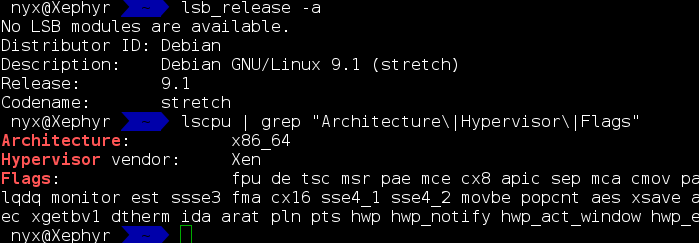
\includegraphics[width=0.75\textwidth]{Figures/sistema-base.png}
    \end{center}
  	\caption{Información del Sistema Base.}
    \label{sistema-base}
\end{figure}

Como se presenta en la figura \ref{sistema-base}, el sistema base para el desarrollo de este trabajo de titulacion utiliza Xen instalado con Debian Stretch (9.1)\footnote{Como el sistema de Dom0} instalado en un LVM con el nombre del grupo de volumenes ''Xephyr-VG''. Originalmente se tenia planificado trabajar con Debian Jessie (8.x) debido que eso fue la version estable al momento de instalacion pero despues se opto por una actualizacion a la version beta de Debian en aquello momento (Debian Stretch). En resumen los pasos realizados fueron:
\lstset{language=Bash}
\begin{enumerate}
	\item Instalacion Limpia de Debian 8 con un LVM.
    	\begin{description}
    		\item[Volumen Fisico:] /dev/sda8 310g 
            \item[Grupo de Volumenes:] Xephyr-VG 310g
            \item[Volumenes Logicos:] Originalmente 4 (se agrega 2 por cada nueva maquina virtual -- uno para su disco y otro para su area de intercambio).
            \begin{description}
            	\item[Xephyr-Dom0] Xephyr-VG 30g
                \item[Xephyr-IMG-Repo] Xephyr-VG 20g
                \item[Xephyr-ISO-Repo] Xephyr-VG 20g
                \item[Xephyr-Swap] Xephyr-VG 4g
            \end{description}
    	\end{description}
    \item Actualizar Instalacion de Debian 8.
    	\begin{lstlisting}
	apt update
	apt upgrade
	apt dist-upgrade
	reboot
        \end{lstlisting}
    \item Actualizar Debian 8 a Debian 9.
        \begin{lstlisting}
	sed -i 's/jessie/stretch/g' /etc/apt/sources.list
	apt update
	apt upgrade
	reboot
        \end{lstlisting}
    \item Instalacion de Herramientas de Trabajo
        \begin{lstlisting}
	apt install tmux vim zsh
        \end{lstlisting}
    \item Instalacion y Configuracion de Hipervisor Xen
		\begin{lstlisting}
	apt install xen-hypervisor
	dpkg-divert --divert /etc/grub.d/08_linux_xen \
		--rename /etc/grub.d/20_linux_xen
	update-grub
	cat > /etc/network/interfaces.d/xenbr << EOF

	auto xenbr0
	iface xenbr0 inet static
		address 10.10.10.1
		netmask 255.255.255.0
		bridge_ports wlan0

	#other possibly useful options in a
	#	virtualized environment
		#bridge_stp off		# disable
		#		Spanning Tree Protocol
		#bridge_waitport 0	# no delay
		#		before a port becomes
		#		available
		#bridge_fd 0		# no forwarding
		#		delay

	## configure a (separate) bridge for
	#	the DomUs without giving Dom0 an
	#	IP on it
	#auto xenbr1
	#iface xenbr1 inet manual
	#   bridge_ports eth1

	EOF

	reboot
		\end{lstlisting}
	\item Instalacion de Herramientas de Xen
		\begin{lstlisting}
	apt install xen-tools xen-utils
		\end{lstlisting}
    \item Instalacion de Herramientas de Desarrollo para Python 3
    	\begin{lstlisting}
	apt install python3 python3-virtualenv python3-pip
    	\end{lstlisting}
\end{enumerate}

Estos pasos de instalacion se basaron en la guia de instalacion de Xen publicado en el wiki del proyecto de Debian \citep{Debian-Wiki-Xen}.

Para dar connexiones hace el exterior a las maquinas virtuales, se necesita activar una regla NAT en el cortafuego IPTables:

\begin{lstlisting}
	iptables -t nat -A POSTROUTING -o wlan0\
    		-j MASQUERADE
\end{lstlisting}

\subsection{Ambiente Virtual de LMS (Moodle)}

Para el ambiente de Moodle (LMS contra el cual se ha llevado el desarrollo), se crea una maquina virtual de Debian Stretch (9) con 1 GiB de RAM, 1 CPU virtual, 6 GiB de disco, 512 MiB de intercambio y una direccion IP fija de 10.10.10.10. Los resultados del mismo commando se puede ver en la figura \ref{vm-moodle}.
\begin{lstlisting}
	xen-create-image --hostname=debian-moodle\
    		--ip=10.10.10.10 --netmask=255.255.255.0\
        	--gateway=10.10.10.1 --memory=1024mb\
        	--vcpus=1 --lvm=Xephyr-VG --pygrub\
        	--dist=stretch --force --size=6144mb\
        	--swap=512mb
\end{lstlisting}

\begin{figure}
	\begin{center}
    	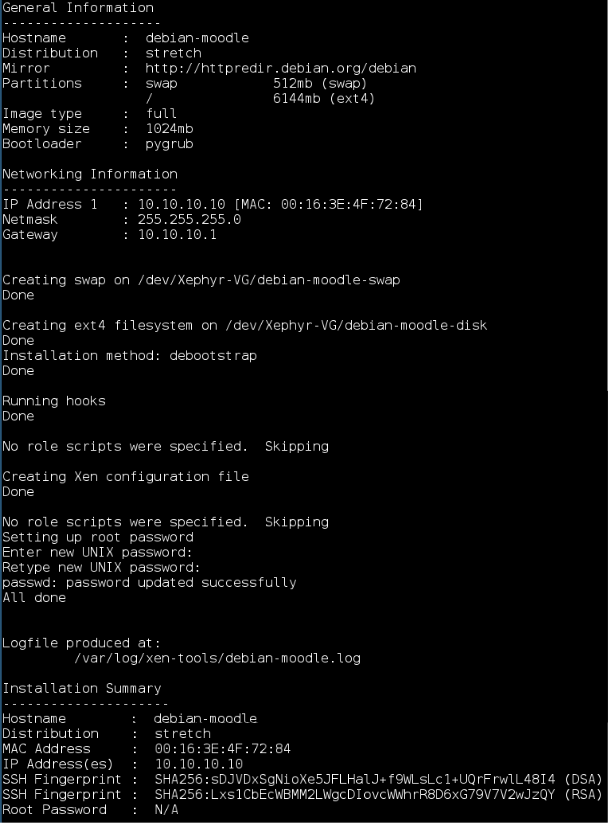
\includegraphics[width=0.75\textwidth]{Figures/crear-moodle.png}
    \end{center}
  	\caption{Crear maquina virtual para Moodle.}
    \label{vm-moodle}
\end{figure}

Se renombró el archivo de configuracion de la maquina virtual generado en el paso anterior para temas de consistencia.

\begin{lstlisting}
	mv /etc/xen/debian-moodle.cfg\
    		/etc/xen/domU-debian-moodle.cfg
\end{lstlisting}

Un bug de Xen-Tools causa que no se instala correctamente un nucleo de Linux en la maquina virtual y por lo tanto es necesario entrar al mismo con un Chroot y instalar los paquetes faltantes (y hacer las adecuadas configuraciones  para permitir su aranque independiente de ayuda externa).

\begin{lstlisting}
	mount /dev/Xephyr-VG/debian-moodle-disk /mnt
	mount -o bind /proc /mnt/proc
	mount -o bind /sys /mnt/sys
	mount -o bind /dev /mnt/dev
	cp /etc/resolv.conf /mnt/etc/resolv.conf
	chroot /mnt /bin/bash
	apt install linux-image-amd64
	vim.tiny /boot/grub/menu.lst
	# Revisar que los archivos referenciados existen
	#		de verdad por ejemplo:
	# Replace initrd.img- con initrd.img
    # guarda y sale
	exit
	umount /mnt/proc            
	umount /mnt/sys 
	umount /mnt/dev 
	umount /mnt	
\end{lstlisting}

Para levantar la maquina virtual:

\begin{lstlisting}
	xl create /etc/xen/domU-debian-moodle.cfg -c
\end{lstlisting}

Se debe selecionar la tercera opcion (Default Kernel).

Se puede dar una revision a la configuracion de red para asegurarse de que esta correcto:

\begin{lstlisting}
	vim.tiny /etc/network/interfaces
\end{lstlisting}

Debe contener:

\begin{lstlisting}
auto eth0
iface eth0 inet static
 address 10.10.10.10
 gateway 10.10.10.1
 netmask 255.255.255.0
\end{lstlisting}

En el presente caso, Xen-Tools logró configurar esta parte de forma correcta.

A continuacion se procede con la instalacion de Moodle:

\begin{lstlisting}
# actualiza el sistema
apt update
apt upgrade

# instala dependencias
apt install apache2 php7.0 mysql-server php7.0-mysql
apt install libapache2-mod-php7.0 php7.0-gd php7.0-curl
apt install php-xml php-zip php-mbstring php-soap
apt install php7.0-xmlrpc php7.0-intl
vim.tiny /etc/php/7.0/apache2/php.ini

# agrega:
extension=mysql.so 
extension=gd.so

# edita:

memory_limit = 40M
# dejado con el valor por defecto de 128M

post_max_size = 80M
upload_max_filesize = 80M

# guarda y sale

# reinicia apache para coger los cambios
systemctl restart apache2

\end{lstlisting}

A continuacion se configura la base de datos:

\begin{lstlisting}

# clave de root es root
mysqladmin -u root password "root"

# logear como root
mysql -u root -p

# crear base de datos y hacer que ocupa UTF-8
mysql> CREATE DATABASE moodle;
mysql> ALTER DATABASE moodle charset=utf8;
mysql> exit;

## No se implemento ##
# Moodle queja de UTF8

# Se podria arreglar
# (antes de instalar Moodle)
# con:

mysql -u root -p

mysql> ALTER DATABASE moodle charset=utf8mb4;
mysql> exit;
######################

systemctl restart mysql

\end{lstlisting}

Se realiza la instalacion de la ultima version de Moodle (3.3 con sus respectivos patches de fallas desde que el mismo salio):

\begin{lstlisting}

# descargar
wget https://download.moodle.org/download.php/direct/stable33/moodle-latest-33.tgz

# descomprimir
tar -zxvf moodle-latest-33.tgz

# meter en ubicacion para apache
mv moodle /var/www

# ir a ubicacion para apache
cd /var/www

# crear ubicacion para datos
mkdir moodledata

# arreglar permisos
chown -R www-data:www-data moodle
chown -R www-data:www-data moodledata
chmod -R 755 moodle
chmod -R 755 moodledata

# modificar configuracion de apache
vim.tiny /etc/apache2/sites-available/000-default.conf

# editar
DocumentRoot "/var/www/moodle"

# guardar y salir

# reiniciar apache para aplicar los cambios
systemctl restart apache2

\end{lstlisting}

Arreglar la base de datos para que acepte conexiones desde Moodle:

\begin{lstlisting}

mysql -u root -p

GRANT ALL PRIVILEGES on *.* to
	'root'@'localhost' IDENTIFIED BY 'root';
GRANT ALL PRIVILEGES on *.* to
	'root'@'localhost' IDENTIFIED BY 'root';
FLUSH PRIVILEGES;
exit;

\end{lstlisting}

Para seguir con la instalacion se abre un navegador con la direccion \url{http://10.10.10.10/} para seguir las instrucciones que se le lleve por toda la configuracion inicial del Moodle.

Al final se agrege un trabajo de cron para ayudar con los tareas periodicas que Moodle requiere para su mantemiento continuo:

\begin{lstlisting}

crontab -u www-data -e
# add line:
*/10 * * * * /usr/bin/php
		/var/www/moodle/admin/cli/cron.php
        		>/dev/null

\end{lstlisting}

Estos pasos fueron adaptados de la guia oficial del proyecto de Moodle para instalacion en Debian \citep{MOODLE-Install-Debian}.

% <TODO>

%%%%%%%%%%%%%%%%%%%%%%%%%%%%%%%%%%%%%%%%%%%%%%%%%%%%
% \subsection{Servidor de Git (GitLab CE)}
%%%%%%%%%%%%%%%%%%%%%%%%%%%%%%%%%%%%%%%%%%%%%%%%%%%%

%%%%%%%%%%%%%%%%%%%%%%%%%%%%%%%%%%%%%%%%%%%%%%%%%%%%
% \subsection{Servidor de Virtualizacion (???)}
%%%%%%%%%%%%%%%%%%%%%%%%%%%%%%%%%%%%%%%%%%%%%%%%%%%%

%%%%%%%%%%%%%%%%%%%%%%%%%%%%%%%%%%%%%%%%%%%%%%%%%%%%
% \subsection{Plantilla de Maquina Virtual (???)}
%%%%%%%%%%%%%%%%%%%%%%%%%%%%%%%%%%%%%%%%%%%%%%%%%%%%

% </TODO>

\section{GitEDU}

La gestion de dependencias del sistema GitEdu se maneja con un entorno virtual y el gestor de paquetes de python pip. El siguiente es un script de bash diseñado a detectar si es que existe el entorno virtual (lo crea en caso de que no existe) y despues instala los requiermientos faltantes como son especificados en un archivo aparte ''requirements.txt'' que da liberias y sus versiones.

\begin{lstlisting}

# run with `source activate.sh` 
if [ ! -d env ]; then
	virtualenv --python=python3 env
fi
source env/bin/activate
pip3 install -r requirements.txt

\end{lstlisting}

El script anterior se ejecuta desde el raiz del repositorio con el comando:

\begin{lstlisting}
source activate.sh
\end{lstlisting}

Con el entorno creado y activado se puede proceder a instalar cualquier dependencia necesaria que no ha sido instalado previamente:

\begin{lstlisting}
pip install <nombre_dependencia>
\end{lstlisting}

Para el presente proyecto se instalaron las siguientes dependencias:
\begin{itemize}
	\item Django (1.10.6)
    \item Psycopg2 (2.7.1)
    \item Python-GitLab (0.20)
\end{itemize}

Con las dependencias instaladas o con cada cambio que se realiza de dependencias se ejecuta el siguiente commando para actualizar la lista de los mismos:

\begin{lstlisting}
pip freeze > requirements.txt
\end{lstlisting}

\subsection{Autenticacion por LTI}

\subsection{Editor de Codigo en Linea}

\subsection{Persistencia de Codigo}

\subsection{Sincronizacion de Notas por LTI}

\subsection{API Externa}

\section{EduNube}

\subsection{Ejeccucion de Codigo en Linea}

\subsection{Calificacion Automatizada con Pruebas Unitarias}

\subsection{API Externa}
